\chapter{Assurance Cases and Selected Evidence for AortaGeomRecon}

\section{Assurance Case Development}

Assurance Case shows the statements and the evidences to ensure the goals are fulfilled. By using Astah System Safety presenting in Goal Structuring Notation (GSN) arguments, we want to show that our software delivers correct outputs when used for its intended use/purpose in its intended environment, and within its assumed operating assumptions. The Figure~\ref{fig_agr_ac_top} shows the top level of the assurance cases. Having the goal of delivering correct outputs, we are decomposing the goal into 4 sub goals, GR, GI, GA and GBA.

\begin{figure}[H]
    \centering
    \fbox{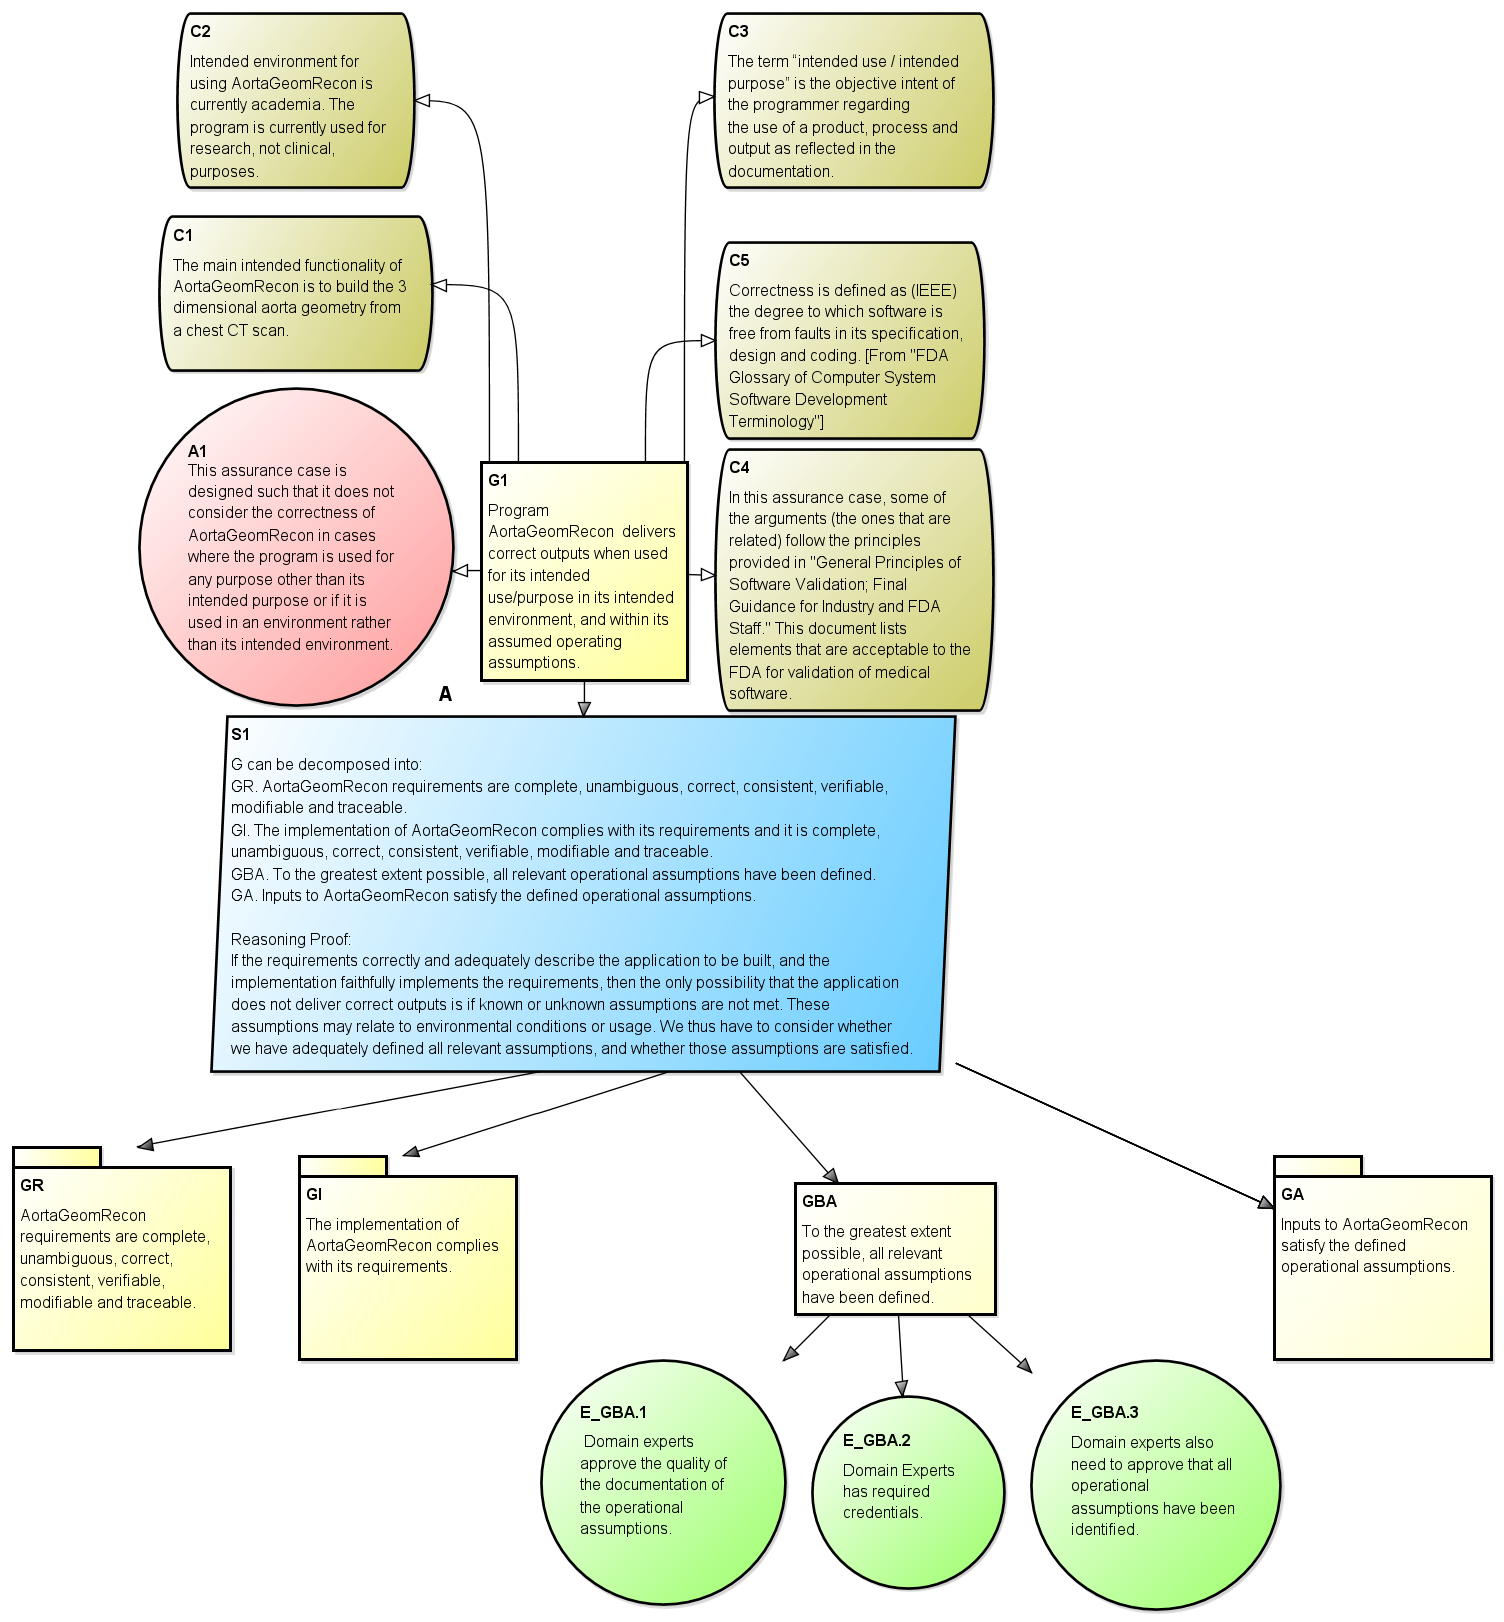
\includegraphics[width=\textwidth]{figures/AC/Top_Level.png}}
    \caption[AortaGeomRecon Assurance Cases Top Level]{AortaGeomRecon Assurance Cases Top Level}
    \label{fig_agr_ac_top}
\end{figure}


\section{Assurance Case for Software Specification Requirements}

The first goal of getting a trusted software is having a complete, unambiguous, correct, consistent, verifiable, modifiable and traceable Software Specification Requirements \citep{SRS} which shows the complete breakdown of the requirements with mathematical notation, data models and instance models. It's the foundation of the software development, and the design and the implementation will be based on the requirement document.


\begin{figure}[H]
    \centering
    \fbox{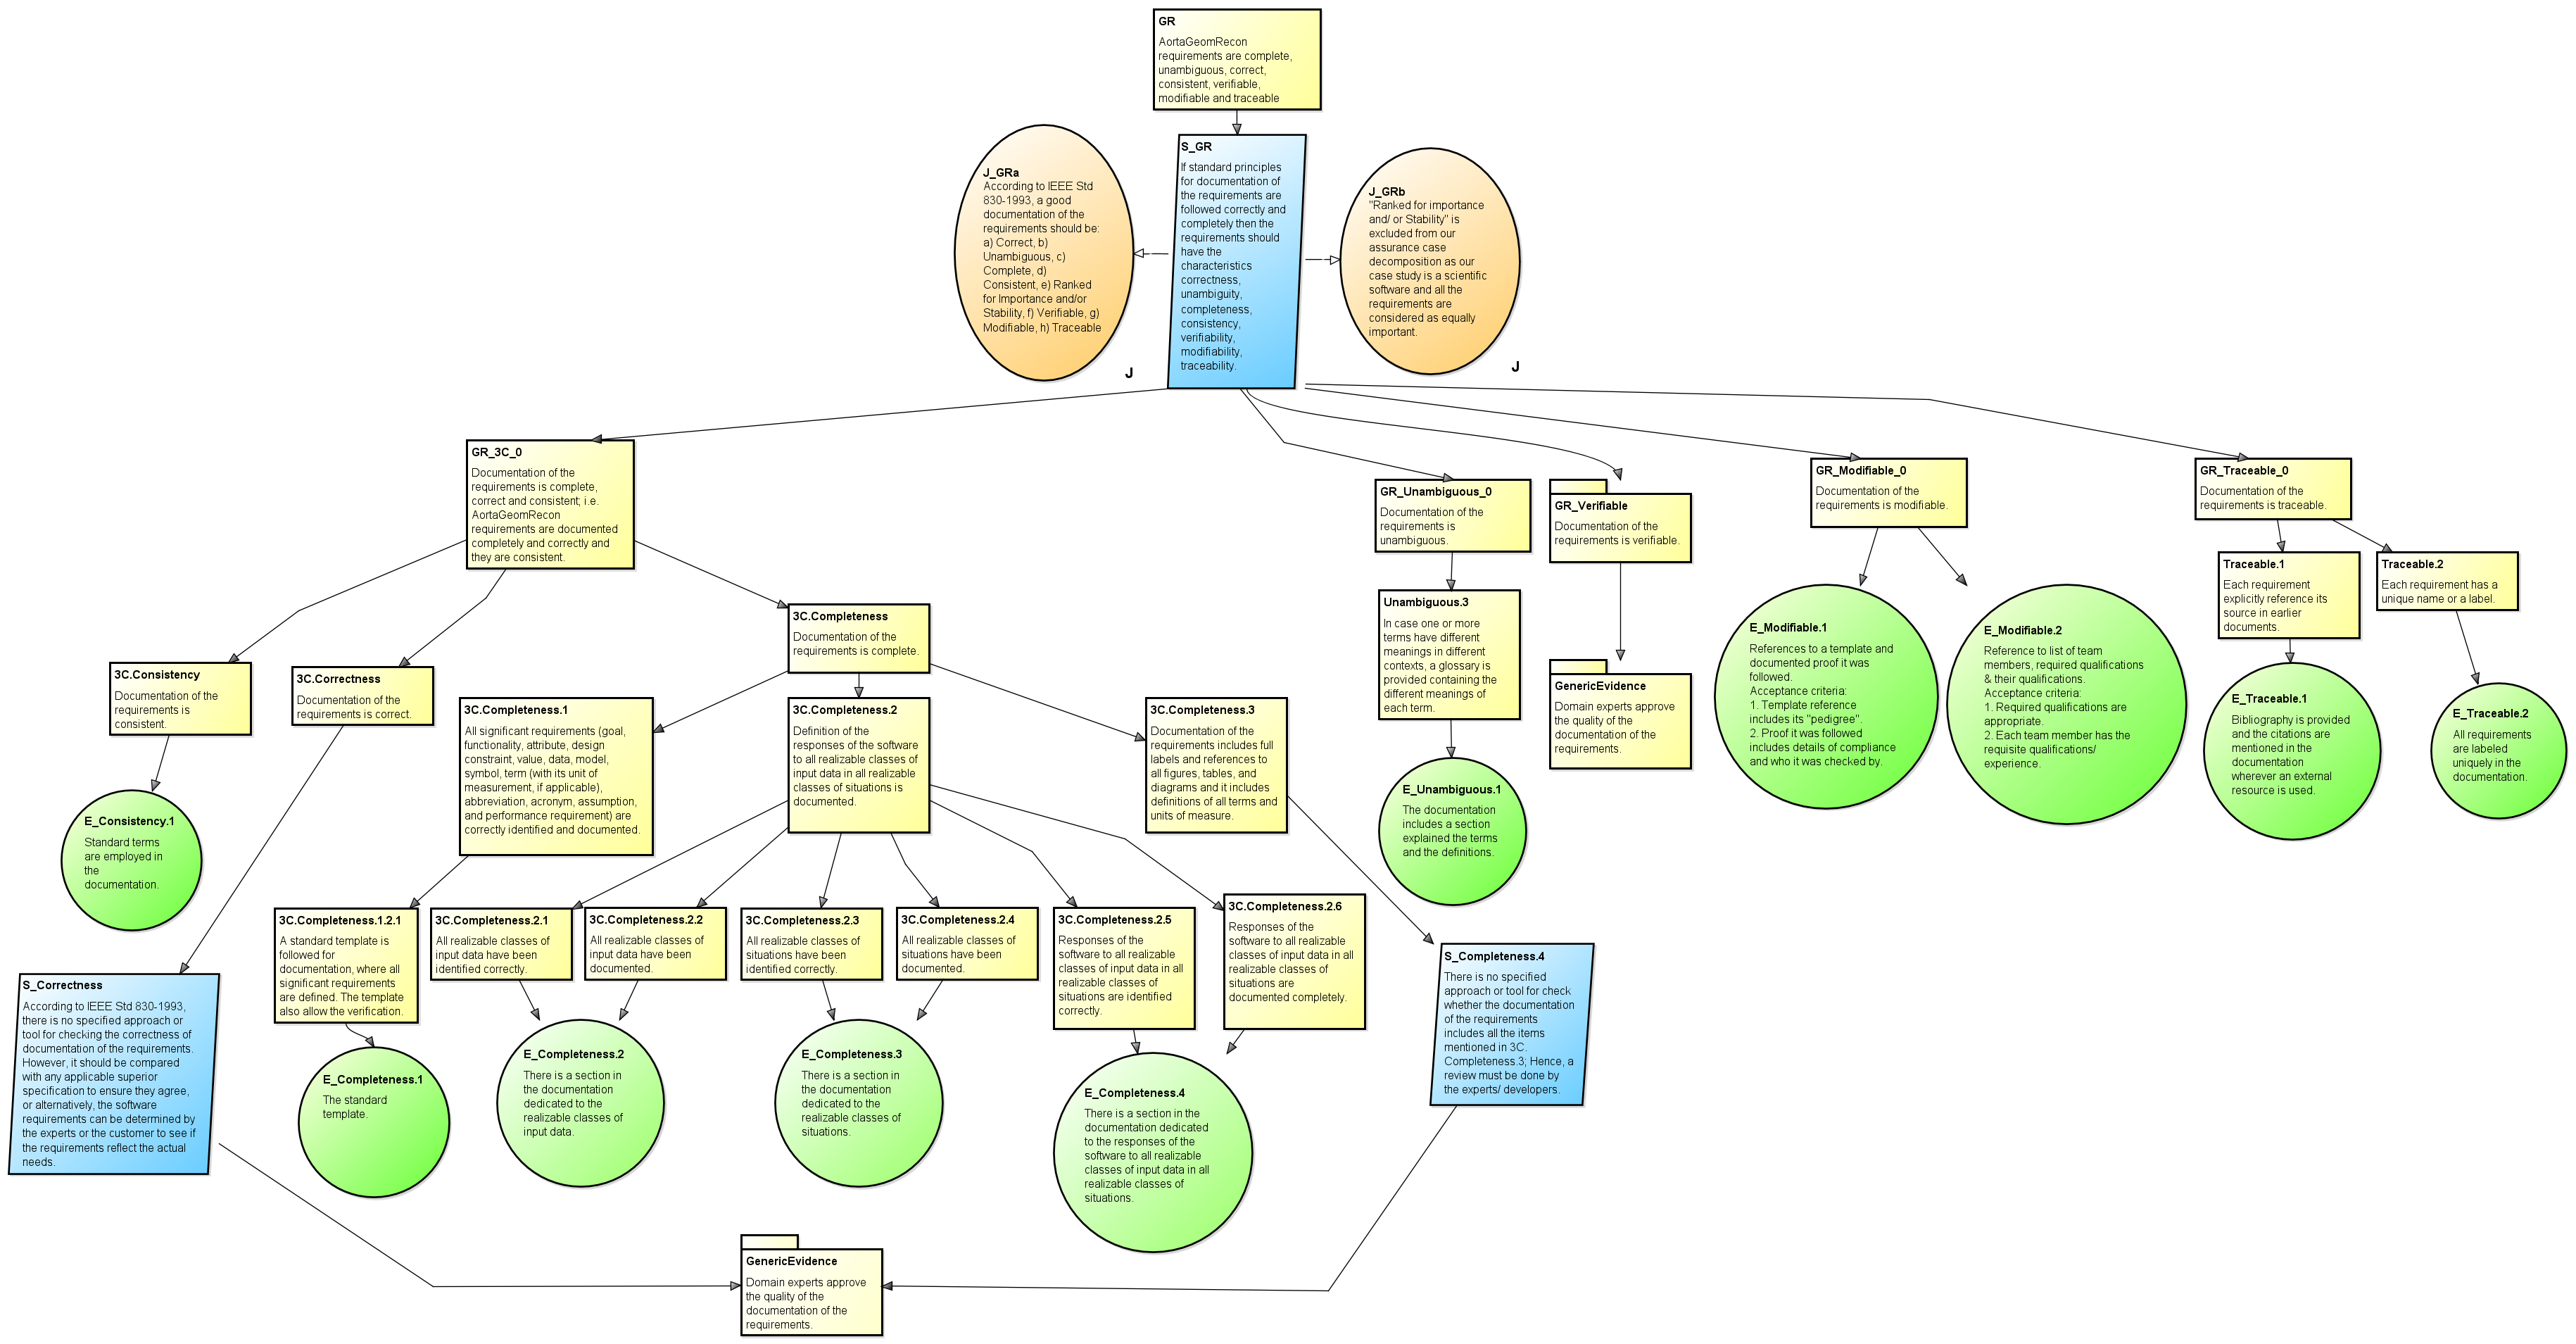
\includegraphics[width=\textwidth]{figures/AC/SRS/GSN_GR.png}}
    \caption[AortaGeomRecon Assurance Cases GR]{AortaGeomRecon Assurance Cases GR}
    \label{fig_agr_ac_gr}
\end{figure}



As explains in the assurance case GR, one of  most important statement of SRS having these characteristics is using a standard template. This template is provided by the domain expert, and my professor, Dr. Spencer Smith, who has researched on Application of Software Engineering Principles, Methods, Techniques and Tools to Improve the Sustainability of Research Software.

The chapters in SRS and some of the most important sections in the chapter are explained below:
\begin{itemize}
\item Reference Material

In this section, a Table of Symbols and an Abbreviations and Acronyms table are used to explain every symbol and Abbreviations used in the SRS document. These tables ensure the consistency and the unambiguous characteristics of the document. They are located at the very beginning of the document, so the reader will firstly look at these tables before reading the entire document.

\item Introduction

In the introduction section, we introduced the problems and the scope of the document to the user by explaining the purpose of document, abstracting the scope of requirements and defining the characteristics of intended reader. 

\item General System Description

The general system description includes a system context diagram which explains the relationship between the users, the inputs given by the user and the outputs of the AortaGeomRecon program. User responsibility and AortaGeomRecon responsibility are defined such that the reader knows what to do to successfully generate the desired result. 

\item Specific System Description

In this section, we are presenting more details about the problem and the specific system to solve the problem. The first subsection Problem Description discussed on the definition of Organ Segmentation, Coordinate Systems used in Medical Image, Physical System Description which is not available, and Goal Statements which is extract the three-dimensional segmentation of the aorta.

In the next subsection, Solution Characteristics Specification, we started with Assumptions to simplify the problem and helps in developing the theoretical model by filling in the missing information for the physical systems. In the subsection Data Definitions, we defined Voxel, Image/Slice, and Volume with mathematical notation so that the developer can easily interpret. Next, in the subsection Instance Model, we showed the mathematical meaning of Region of Interest, and Segmentation, which are the two essential terms that the developer must know in order to develop the solution.


\begin{figure}[H]
    \centering
    \fbox{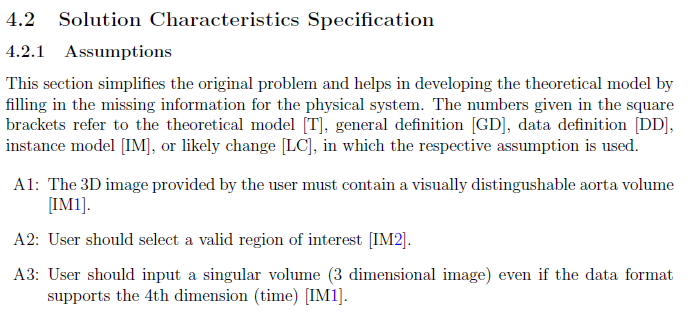
\includegraphics[width=\textwidth]{figures/AC/SRS/Assumptions.png}}
    \caption[AortaGeomRecon SRS Assumptions]{AortaGeomRecon SRS Assumptions}
    \label{fig_agr_srs_a}
\end{figure}


\item Requirements

With all the information in the document, we can now present the Functional Requirements and the Non-Functional Requirements for the program AortaGeomRecon. The Functional Requirements are defined By using the terms we presented in Data Definitions, Instance Model, and based on the other Functional Requirements. The Non-Functional Requirements usually have a measurement such as execution time, the effort of manual works, etc.

\begin{figure}[H]
    \centering
    \fbox{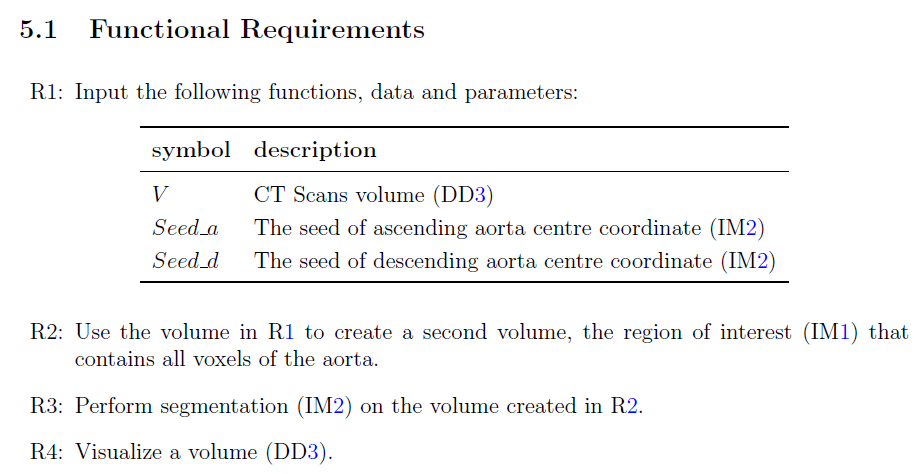
\includegraphics[width=\textwidth]{figures/AC/SRS/Functional_Requirements.png}}
    \caption[AortaGeomRecon Functional Requirements]{AortaGeomRecon Functional Requirements}
    \label{fig_agr_fr}
\end{figure}

\begin{figure}[H]
    \centering
    \fbox{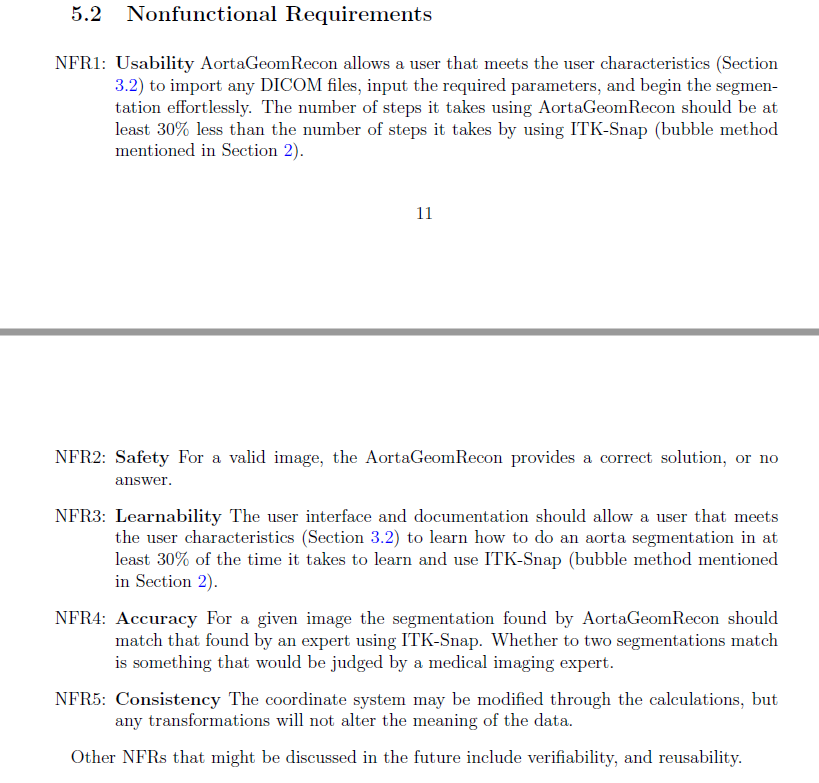
\includegraphics[width=\textwidth]{figures/AC/SRS/NonFunctional_Requirements.png}}
    \caption[AortaGeomRecon Non- Functional Requirements]{AortaGeomRecon Non- Functional Requirements}
    \label{fig_agr_nfr}
\end{figure}

\item Likely Changes and Unlikely Changes

This section discussed the likely changes that the developer might expect a change in the future works, and the unlikely changes that is most certainly not going to change for a justified reason. The only likely change discussed in the AortaGeomRecon's SRS is regarding the segmentation method. For different segmentation method, the inputs varies, since the segmentation method is a likely change, the inputs variables are also likely changes. The only unlikely change is the method of retrieve a region of interest. Most methods take a starting point and sizes in different dimensions to get the region of interest.

\item Traceability Matrix and Graphs

The traceability matrices are to provide easy references on what has to be additionally modified if a certain component is changed. Below shows the traceability matrices of different sections:
\begin{figure}[H]
    \centering
    \fbox{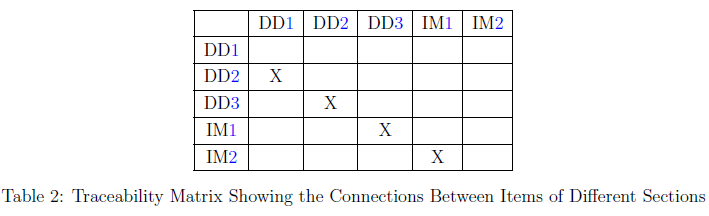
\includegraphics[width=\textwidth]{figures/AC/SRS/tm_dd_im.png}}
    \caption[AortaGeomRecon Traceability Matrix between Data Definitions and Instance Model]{AortaGeomRecon Traceability Matrix between Data Definitions and Instance Model}
    \label{fig_agr_tm_dd_im}
\end{figure}

\begin{figure}[H]
    \centering
    \fbox{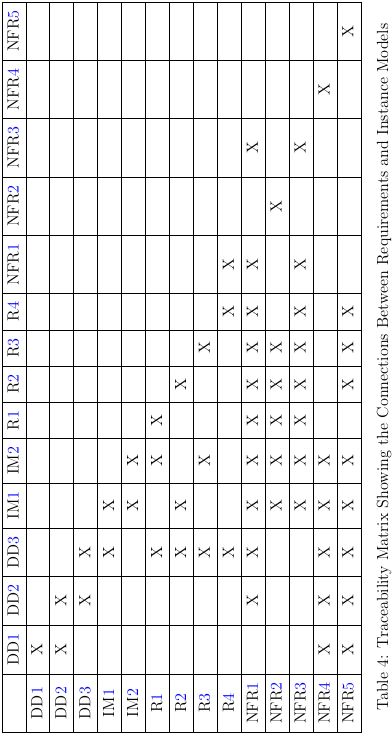
\includegraphics[width=\textwidth]{figures/AC/SRS/tm_im_r.png}}
    \caption[AortaGeomRecon Traceability Matrix between Requirements and Other sections]{AortaGeomRecon Traceability Matrix between Requirements and Other sections}
    \label{fig_agr_tm_im_r}
\end{figure}

\begin{figure}[H]
    \centering
    \fbox{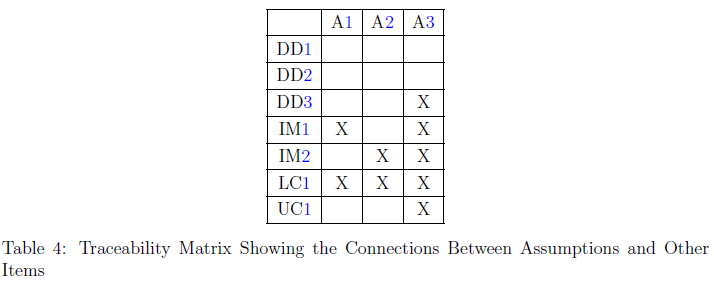
\includegraphics[width=\textwidth]{figures/AC/SRS/tm_a.png}}
    \caption[AortaGeomRecon Traceability Matrix between Assumptions and Other sections]{AortaGeomRecon Traceability Matrix between Assumptions and Other sections}
    \label{fig_agr_tm_a}
\end{figure}


\end{itemize}

\section{Assurance Case for Implementation}
The goal of implementation asked the developer to fully comply the design and the implementation with the Software Requirements Specification document. Since we have showed with Assurance Case that our SRS is complete, consistent, and unambiguous, the design and the implementation that fully complying with requirements is correct.

\begin{figure}[H]
    \centering
    \fbox{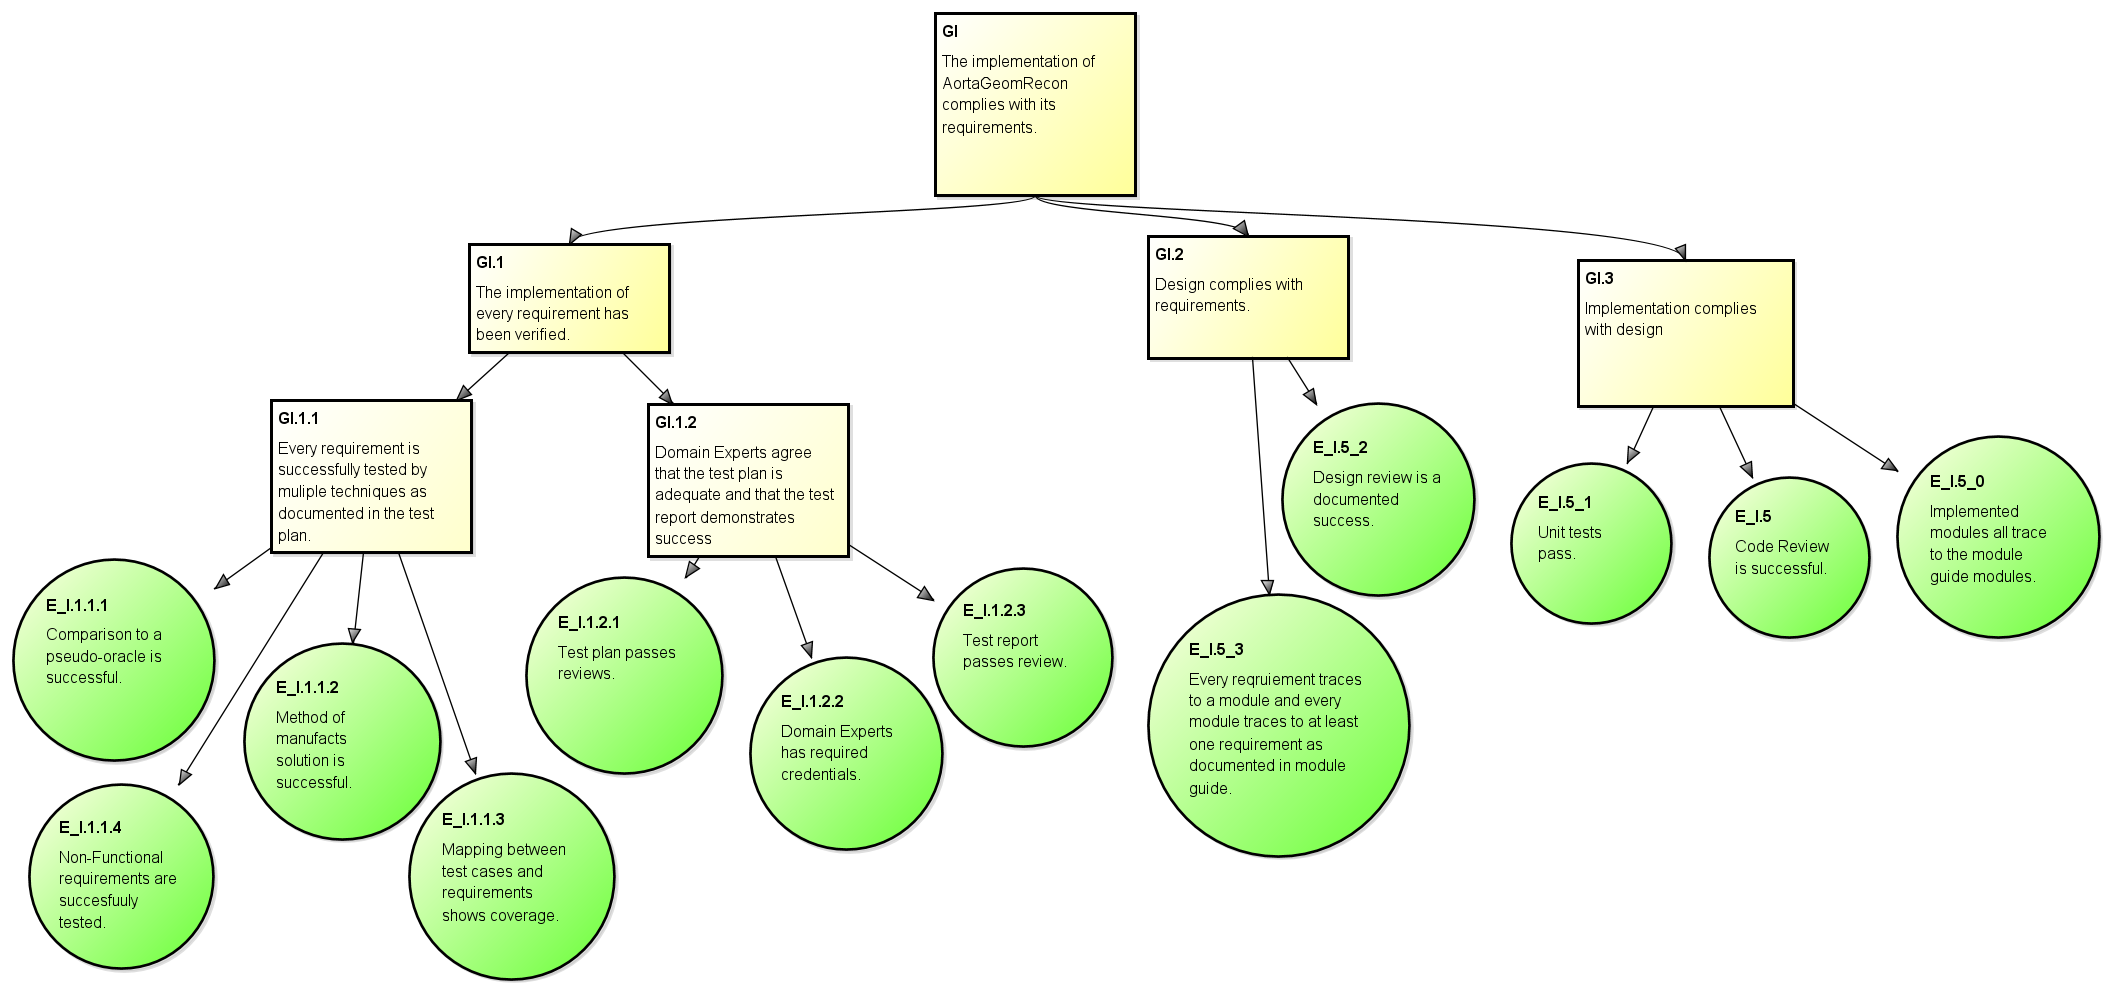
\includegraphics[width=\textwidth]{figures/AC/GI/GSN_GI.png}}
    \caption[AortaGeomRecon Assurance Cases for Implementation]{AortaGeomRecon Assurance Cases for Implementation}
    \label{fig_agr_ac_gi}
\end{figure}

\subsection{Design Document}
The purpose of the Design Document is to explain in details how the algorithm works, and why it worked. Similar to what section \ref{algo} wrote, the design document explains in plan text the workflow of the algorithm. Since before the domain expert can agree on the design and implementation, the person needs to understand the algorithm, we are building a Design Document that is easy to access. 

\subsubsection{Sphinx - Python Documentation Generator}
To implement this Design Document, I used Sphinx, a Python Documentation Generator that can build module's documentation with the comments in the source code. Moreover, using reStructuredText to write the Algorithm Overview, we can build HTML binary which can be published on a web server, which I was able to implement and accomplish. Another important section in Design Document is the Glossary. It has rich vocabulary explanation, images, and links to the outside source to let the reader understands as much as possible.

\begin{figure}[H]
    \centering
    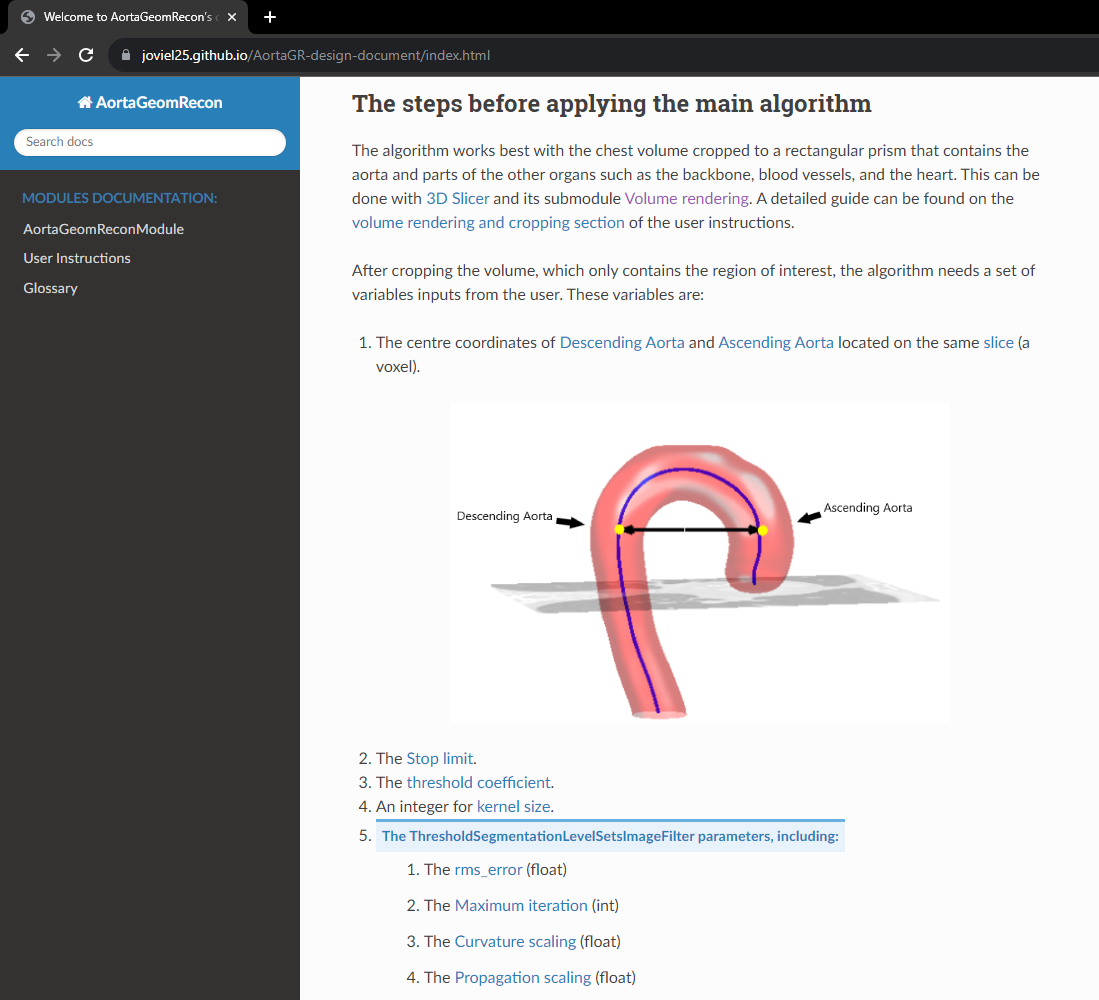
\includegraphics[width=\textwidth]{figures/AC/DD/Main_page.png}
    \caption[AortaGeomRecon Design Document website]{AortaGeomRecon Design Document website}
    \label{fig_agr_dd}
\end{figure}

\begin{figure}[H]
    \centering
    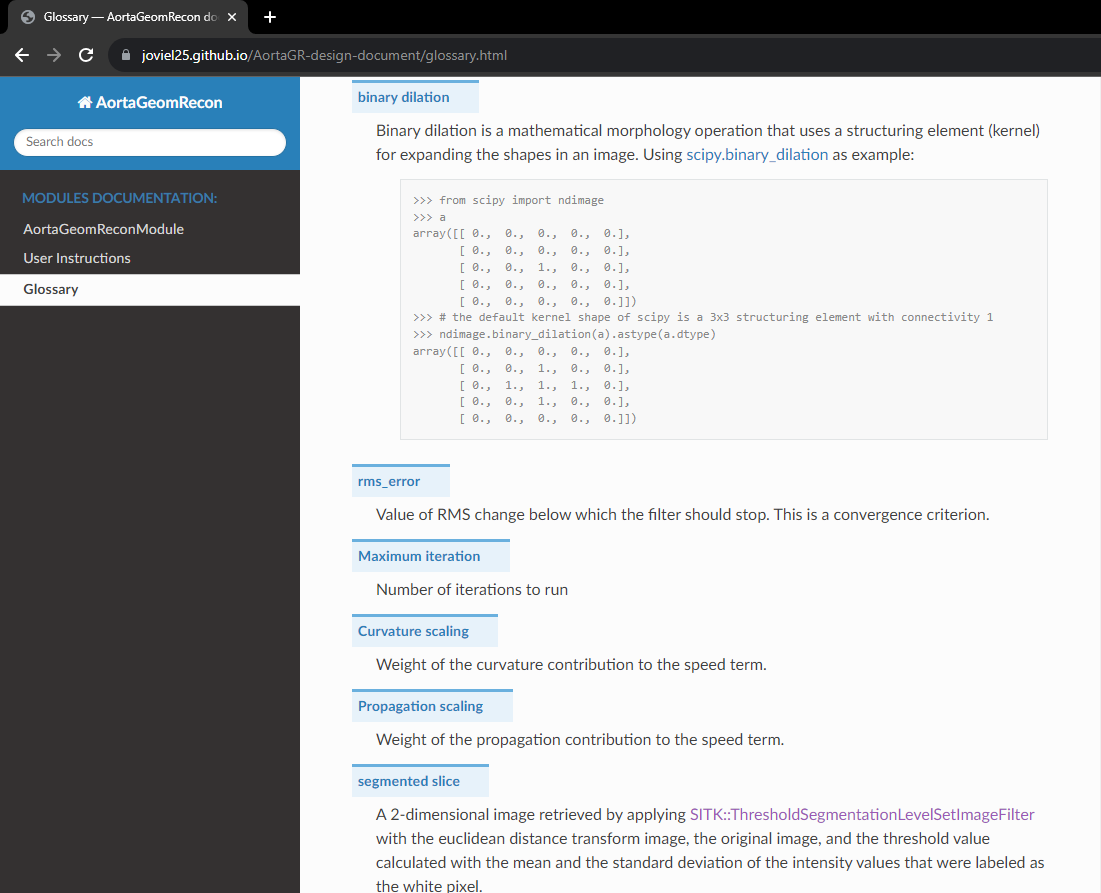
\includegraphics[width=\textwidth]{figures/AC/DD/Glossary.png}
    \caption[AortaGeomRecon Design Document Glossary]{AortaGeomRecon Design Document Glossary}
    \label{fig_agr_dd_glossary}
\end{figure}

\subsection{Module Guide}

In the design of the software, we first list the anticipated changes such that since we are expecting a change to this piece of requirement of information, we will keep it a single module so when the changes did happen, we only need to concern about the module and its dependency modules. The anticipated changes are listed in the Figure~\ref{fig_agr_ac} below.

\begin{figure}[H]
    \centering
    \fbox{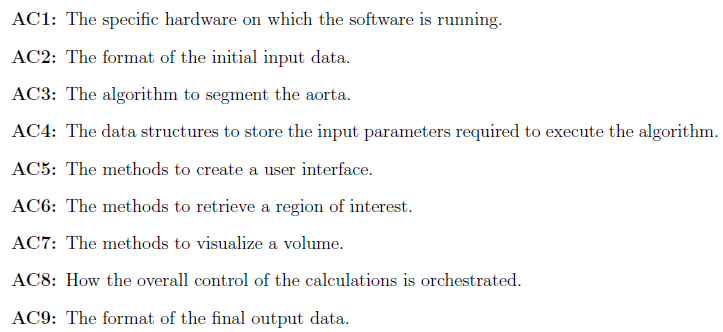
\includegraphics[width=\textwidth]{figures/AC/MG/Anticipated_Changes.png}}
    \caption[AortaGeomRecon Anticipated Changes]{AortaGeomRecon Anticipated Changes}
    \label{fig_agr_ac}
\end{figure}

Modules are decomposed according to the principle of “information hiding” proposed by Parnas et al. (1984). The Secrets field in a module decomposition is a brief statement of the design decision hidden by the module. The Services field specifies what the module will do without documenting how to do it. For each module, a suggestion for the implementing software is given under the Implemented By title. If the entry is OS, this means that the module is provided by the operating system or by standard programming language libraries. AortaGeomRecon means the module will be implemented by the AortaGeomRecon software.

\begin{figure}[H]
    \centering
    \fbox{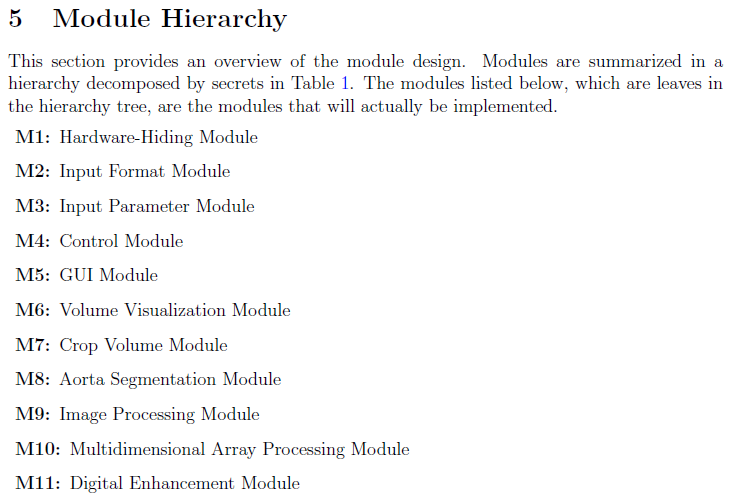
\includegraphics[width=\textwidth]{figures/AC/MG/Modules.png}}
    \caption[AortaGeomRecon Modules]{AortaGeomRecon Modules}
    \label{fig_agr_modules}
\end{figure}

\begin{figure}[H]
    \centering
    \fbox{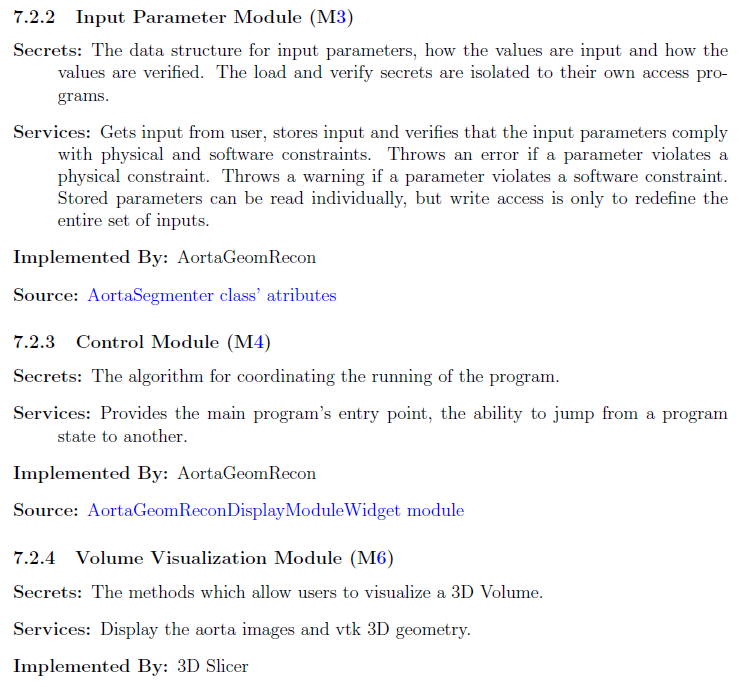
\includegraphics[width=\textwidth]{figures/AC/MG/Modules_Decomposition.png}}
    \caption[AortaGeomRecon Module Decomposition Example]{AortaGeomRecon Module Decomposition Example}
    \label{fig_agr_md}
\end{figure}

Now that we have listed the anticipated changes and the modules, we are using traceability matrices to show the relationships between the modules and the anticipated changes, and the modules between the requirements. This indicates that the design is fully complying with the requirements, as we stated in GI.2 in the Figure~\ref{fig_agr_ac_gi}.

\begin{figure}[H]
    \centering
    \fbox{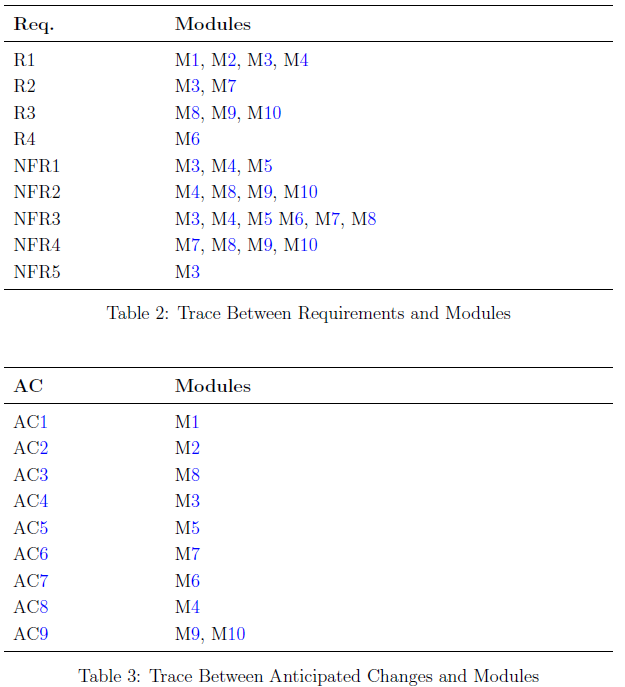
\includegraphics[width=\textwidth]{figures/AC/MG/TM.png}}
    \caption[AortaGeomRecon Modules Traceability Matrices]{AortaGeomRecon Modules Traceability Matrices}
    \label{fig_agr_mtm}
\end{figure}

On top of relating the modules to the requirements, we are relating the actual source code to the modules, which is a strong evidence of our implementation has fully complying with the requirements. Since our requirements has proven to be correct, complete, and consistent, the implementation must also be trustworthy.

\begin{figure}[H]
    \centering
    \fbox{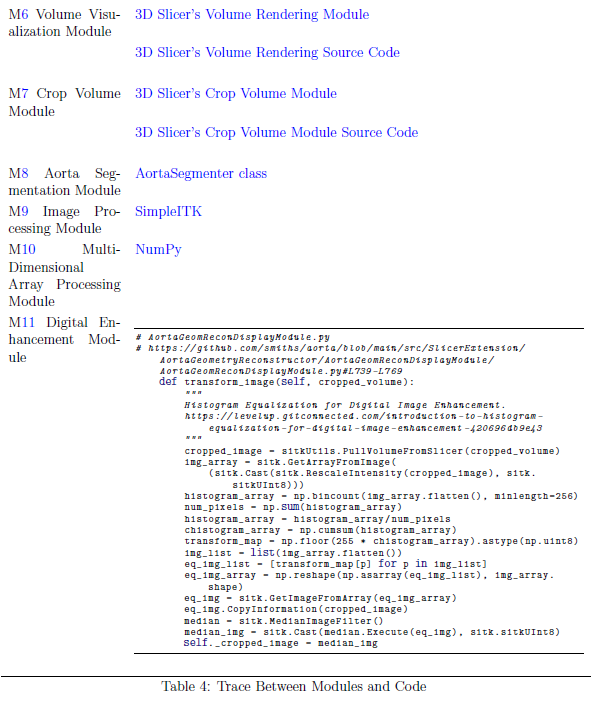
\includegraphics[width=0.9\textwidth]{figures/AC/MG/TM_modules_code.png}}
    \caption[AortaGeomRecon Part of the Traceability Matrix on Modules and Code]{AortaGeomRecon Part of the Traceability Matrix on Modules and Code}
    \label{fig_agr_mtm_modules_code}
\end{figure}

\subsection{Test Plan}

GI.1.2
\begin{itemize}
\item GitHub Workflow
\item Continuous Integration tests
\begin{itemize}
\item build ``Ground Truth Data''
\item Steps
\item Coverage
\end{itemize}
\end{itemize}

\section{Algorithm Review}

The algorithm review was an idea started with Code Walkthrough. The difference is that Code Walkthrough aims to increase the confidence of the reviewer such that the reviewed implementation is doing what we have discussed. For an Algorithm Review, we have not discussed what the program should do; we are presenting the algorithm to the domain expert and asking them if the design and implementation fulfill the implementation objectives.

\subsubsection{Tools used in Algorithm Review}


\begin{itemize}
\item 
\item 
\item 
\end{itemize}

\subsection{Algorithm Review with Kailin Chu}
The first algorithm review was done with Kailin Chu, who is a biomedical engineer and started the semi-automacial aorta segmentation algorithm. Along with Smith Spencer, we were aiming to increase the domain expert's confidence in this code walkthrough. For various reasons, this code walkthrough has not been successful, this implies that the domain expert has not gained confidence over the implementation. However, this meeting was helpful, because knowing that the algorithm might have flaws, I was able to iterate the algorithm and reaching a better result in a more efficient way.

\subsection{Algorithm Review with Dr. Dean Inglis}

The second algorithm review was done with Dr. Dean Inglis, who is an experienced professor, Medical Image Analyst and Software Developer. We showed him our segmentation algorithm and asked for a confirmation of this method, or a better algorithm.





%\section{Referencing}
%These are some sample references to GAMYGDALA~\citep{popescu2014gamygdala} from 
%the \texttt{references.bib} file and state effects of 
%cognition~\citep{hudlicka2002time} from the \texttt{references\_another.bib} 
%file. These references are not in the same .bib file.
%
%\section{Figures}
%This is a single image figure (Figure~\ref{fig_singleenv}):
%
%\begin{figure}[ht]
%    \centering
%    
\includegraphics[width=0.6\textwidth]{figures/Sample/tumblr_static_eaceks0rfxsss8o4swscw40wo.jpg}
%    \caption[Single Figure Environment Listed Title]{This is a single figure 
%    environment}
%    \label{fig_singleenv}
%\end{figure}
%
%This is a multi-image figure with a top (Figure~\ref{fig_multienv_1}) and bottom (Figure~\ref{fig_multienv_2}) aligned subfigures:
%
%\begin{figure}[ht]
%	\centering
%	\begin{subfigure}[t]{\textwidth}
%		\centering
%		
%
\includegraphics[width=0.7\textwidth]{figures/Sample/tumblr_static_eaceks0rfxsss8o4swscw40wo.jpg}
%		\caption{Figure 1}
%		\label{fig_multienv_1}
%	\end{subfigure}
%	~
%	\begin{subfigure}[t]{\textwidth}
%		\centering
%		
%
\includegraphics[width=0.7\textwidth]{figures/Sample/tumblr_static_eaceks0rfxsss8o4swscw40wo.jpg}
%		\caption{Figure 2}
%		\label{fig_multienv_2}
%	\end{subfigure}
%	
%	\caption{A Multi-Figure Environment}
%	\label{fig_multienv}
%\end{figure}
%
%\section{Tables}
%
%Here is a sample table (Table~\ref{tab_sample}):
%
%	\begin{table}[ht]
%	\centering
%	\begin{tabular}{ m{0.2\textwidth} m {0.1\textwidth} m{0.15\textwidth} }
%		\toprule
%		A & $\longleftrightarrow$ & B \\
%		C & $\longleftrightarrow$ & D \\
%		\bottomrule	
%	\end{tabular}	
%	\caption{A sample table}	
%	\label{tab_sample}
%\end{table}
%
%\subsection{Long Tables}
%A sample long table is shown in Appendix~\ref{appendix_b}.
%
%\section{Equations}
%
%Here is a sample equation (Equation~\ref{eq_lineslope}):
%
%\begin{equation} \label{eq_lineslope}
%	y = mx + b
%\end{equation}